\documentclass[]{article}

\usepackage{amsmath}  % AMS math package
\usepackage{amssymb}  % AMS symbol package
\usepackage{bm}       % bold math
\usepackage{graphicx} % Include figure files
\usepackage{dcolumn}  % Align table columns on decimal point
\usepackage{multirow} % Multirow/column tables
\usepackage{hyperref} % Hyperlinks
\usepackage{float}

\begin{document}

\title{Molecular Dynamic Simulation of Argon using 3D Face Centered Cubic Lattice}% Force line breaks with \\
\author{Thavappiragasam Mathialakan}
\date{\today}% It is always \today, today, but you can specify other dates manually 
\maketitle

\begin{abstract}
The MD analyzing approach obviously deals with mass data to study the behavior of material and energy related with temperature. This analysis could be worked out in FCC lattice with periodic boundary condition. In this paper, we implement and analysis the MD method for Argon gas using C++ coding and Excel graphs. 
\end{abstract}


\section{Introduction} %Title for the section
\label{sec:level1} %Label for the section, to be used for referencing in other parts of the document

Molecular Modeling is concerned with the description of the atomic and molecular interactions that govern microscopic and macroscopic behaviors of physical systems. MD (Molecular dynamics) programs simulate the behavior of biomolecular systems, leading to understanding of their functions. The method allows the prediction of the static and dynamic properties of substances directly from the underlying interactions between the molecules.  Classical MD simulations of molecular systems involves the solution of Newton's equations of motion in small time steps, based on Cartesian coordinates of the particles and using a conservative force field (equation ~\ref{eq:one}). The force is found from a potential. The Lennard-Jones potential is an important inter-atomic potential and it is expressed in equation ~\ref{eq:two}. 

\begin{equation}
\label{eq:one}
F = ma = m\frac{d^2r}{dt^2}
\end{equation}

\begin{equation}
\label{eq:two}
V(r) =4\epsilon({(\frac{\sigma}{r})}^{12} - {(\frac{\sigma}{r})}^6)
\end{equation}

where r is the distance between the centers of the two atoms, $\epsilon$ is the strength of the potential energy, and $\sigma$ is the value of r at which the energy is zero. The terms $\frac{1}{r^{12}}$ and $\frac{1}{r^6}$ represent a repulsive hard core interaction between atoms and an attractive dipole-dipole (van der Waals) interaction between the non-polar atoms respectively. This potential is accurate for inert gases. So, It can be adoptable for such an inert gas argon. Argons atoms behave approximately like hard spheres which attract one another with weak van der Waals forces. The forces between two argon atoms can be approximated by this potential energy function (equation ~\ref{eq:two}). In this way, the Lennard-Jones force will be, 

\begin{equation}
\label{eq:three}
F(r) = -  \frac{dV(r)}{d(r)} = \frac{24\epsilon}{\sigma}(2{(\frac{\sigma}{r})}^{13} - {(\frac{\sigma}{r})}^7)
\end{equation}

\subsection{\label{sec:level1.1} Force and Acceleration of an atom}
The non-bonded force calculation is based on a pair list which is updated every \texttt{n} steps. Particles are grouped in charge groups containing one or a few particles. The criterion for inclusion in the list is whether the centers of the charge groups are within a given cut-off radius. This procedure avoids the 'creation' of charges from neutral groups by applying a cut-off criterion to individual pairs of partially charged atoms.
When we chose $\epsilon = 1$, $\sigma = 1$, and mass $m=1$, the vector forces between atoms with positions $r_i$ and $r_j$ will be given by
\begin{equation}
\label{eq:four}
F_{ij} = - F_{ji} = 24(r_i-r_j)(2{(\frac{1}{r})}^{-14} - {(\frac{1}{r})}^{-8})
\end{equation}

where $r=|r_i-r_j|$, and the aceleration for atom $i$ is
\begin{equation}
\label{eq:five}
a_i(t) = \frac{d^2r_i(t)}{dt^2} = \frac{1}{m}\sum_{j=1 j\neq i}^N{F_{ij}}
\end{equation}

\subsection{\label{sec:level1.2} Velocity Verlet Algorithm}
There are many algorithms which can be used to solve ODE’s. This is one of the algorithm was developed by Verlet for the velocity used in MD simulations. The following equations, ~\ref{eq:six} and ~\ref{eq:seven}, derived from Newton's force law and simplified using discrete approximation, Taylor series. It only involves the previous time and a trick central difference on the interval between $t$ and $t+\delta$

\begin{equation}
\label{eq:six}
x_i(t+\delta t) = x_i(t) +v_i(t)\delta t+ \frac{1}{2}a_i(t)\delta t^2
\end{equation}

\begin{equation}
\label{eq:seven}
v_i(t+\delta t) = v_i(t) + \frac{1}{2}[a_i(t+\delta t)+a_i(t)]\delta t
\end{equation}

\subsection{\label{sec:level1.3} The Temperature}
This is a simulation in which the number of particles N and the volume $L^3$ of the system are fixed. Because the Lennard-Jones force is conservative, the total energy of the system is also constant.
If the system is in thermal equilibrium, then Boltzmann$^’s$ Equipartition Theorem gives the absolute temperature \texttt{T} related with kinetic energy,

\begin{equation}
\label{eq:ss3}
T = \frac{2}{3k_B(N-1)}<\frac{m}{2} \sum_{i=1}^N{{v_i}^2}> 
\end{equation}


\section{Algorithm and Techniques used}

\subsection{\label{sec:level2.1}  Algorithm}
This algorithm runs with FCC lattice with periodic boundary condition. It uses the Verlet approach and kinetic energy equation to calculate velocity and temperature respectively. Both the velocity and temperature are measured for a given number of iterations. The random numbers for velocities are generated using Box-Muller algorithm based on Gaussian probability distribution. Boltzman factor $k_B$ is taken as 1.

\texttt{Major Steps of the Algorithm}
\begin{enumerate}
\item Initialize the structure in FCC lattice
\item Find the initial velocities and make zero center of mass momentum
\item Do this for a given number of iterations
\begin{enumerate}
    \item Calculate Verlet velocities using the accelerations $a_i(t)$, $a_i(t+\delta t)$ and applying periodic bounderic condition.
    \item Calculate the temperature using the kinertic energy equation.
    \item Rescale velosity by $\lambda$ if it is the set period
\end{enumerate}

\end{enumerate}

\subsection{\label{sec:level2.2} Face Centered Cubic}
In FCC the lattice points are on the faces of a cube. Each point gives exactly one half contribution ($6*1/2 = 3$) in addition to the corner lattice points ($8*1/8 = 1$). Therefore there are four lattice points per a unit cell.
For a dense system, the atoms are usually placed at the vertices of a face-centered cubic lattice, which tends to minimize the potential energy. The atoms are also given random velocities to approximate the desired temperature. In this work we put the system in a cubical volume of side L and place the particles at the vertices of a simple cubic lattice.
The minimum energy configuration of this Lennard-Jones system is an FCC lattice. This has 4 lattice sites in each conventional cubic unit cell. If the number of atoms $N = 4L_i^3$, where $L_i = 1,2,3,...,$ then the atoms can fill a cubical volume. So MD simulations are usually done with $32 (= 4*2^3), 108 (= 4*3^3), 256, 500,...$ atoms.
The figure shows a conventional cubical unit cell

\begin{figure}[H]
  \centering
  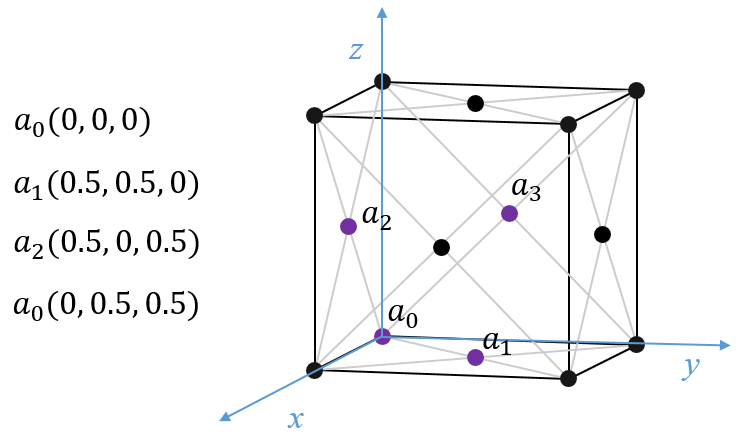
\includegraphics[width=10cm,height=6cm]{figures/Fcc_Cubic}
  \caption{\label{fig:FCC} A cubical unit cell that has four atoms in FCC model }
\end{figure}

The 4 atoms shown in purple provide a basis for the conventional cell. Their positions in units (0, 0, 0)	(0.5, 0.5, 0)	(0.5, 0, 0.5)	(0, 0.5, 0.5) .
	
\subsection{\label{sec:level2.3} Zero center of Mass Momentum}
Since velocities are randomly distributed around zero, the total momentum of the system will be close to zero but not exactly zero. To prevent the system from drifting in space, the center-of-mass velocity (equation ~\ref{eq:eight}) is computed and used to transform the atom velocities to the center-of-mass frame of reference. Then the velocities are scaled by $\lambda$ (equation ~\ref{eq:nine})

\begin{equation}
\label{eq:eight}
Vcm = \frac{\sum_{i=1}^N{mv_i}}{\sum_{i=1}^N{m}}
\end{equation}

\begin{equation}
\label{eq:nine}
\lambda =\sqrt{ \frac{3(N-1)k_BT}{\sum_{i=1}^N{m{v_i}^2}}}
\end{equation}

\subsection{\label{sec:level2.4} Periodic Boundary Condition}

The volume is not really constant because the particles can move out of it. We need to impose suitable boundary conditions to avoid adverse boundary effects, periodic (but not necessarily cubic) boundary conditions are employed.

\section{Implementation}
The high-level programming language C is the most preferable language to deal with mass data, and C++ is an advanced version of C. So, we chose C++ to implement this MD simulation using the approaches as described above. Since 1D array offers better memory locality and less allocation and deallocation overhead, It is faster way than 2 or more dimension for dense matrices. As the reason given above, the data structure 1D integer array is chosen to keep relevant data such as velocity, acceleration, etc.  

\section{Results and Discussion}
In our testing case, 64 atoms are taken in an FCC lattice, and initially they are set with center of mass velocity. We applied the periodic BC boundary condition. The Verlet velocity and temperature are calculated for every iteration. This task is processed for 1000 iterations. The figure ~\ref{fig:Temp_time} shows the changes on temperature with time. You can see a sudden change in 200, it also can be seen in the graph of energy changes (figure ~\ref{fig:chEng}). This energy might be consumed for material change.

\begin{figure}[h]
  \centering
  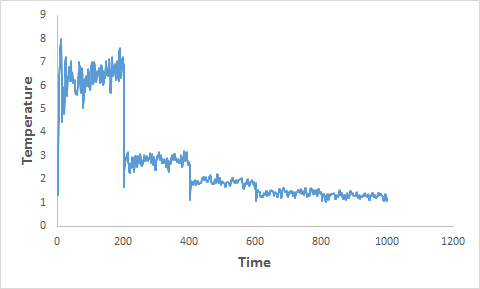
\includegraphics[width=10cm,height=5cm]{figures/Temp_time}
  \caption{\label{fig:Temp_time} Temperature as a function of time.}
\end{figure}

\begin{figure}[h]
  \centering
  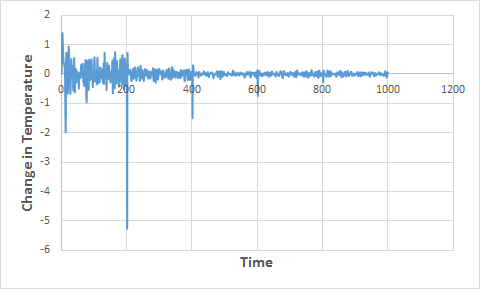
\includegraphics[width=10cm,height=5cm]{figures/chTemp}
  \caption{\label{fig:chTemp} Change in Temperature as a function of time.}
\end{figure}

\begin{figure}[h]
  \centering
  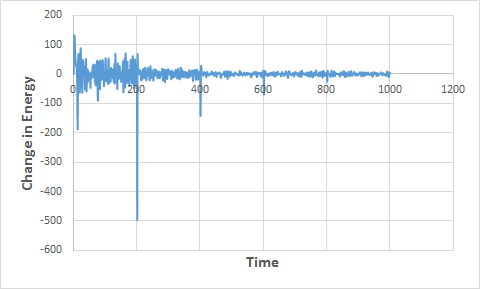
\includegraphics[width=10cm,height=5cm]{figures/chEng}
  \caption{\label{fig:chEng} Change in Energy as a function of time.}
\end{figure}

The specific heat capacity is related with the energy and temperature changes as given in the equation ~\ref{eq:ten}
\begin{equation}
\label{eq:ten}
C = \frac{Q}{m\delta t}
\end{equation}

We took $m=1$, kinetic energy is taken to calculate the energy changes $(v_2^2-v_1^2)/2$, and found C is 47.25.
Particle distribution functions are important objects for investigating the statistical mechanical properties of interacting particle systems. Among them, the two-body (pair) distribution function is very useful, which is defined by

\begin{equation}
\label{eq:eleven}
g(r) = \frac{V}{N^2} \sum_{i=k}{\sum{<\delta(r-r_i-r_k)>}}
\end{equation}

and the $\delta$ function is replaced by
\begin{equation}
\label{eq:twelve}
g(r) = \frac{1}{{2\pi \epsilon^2}^3/2} exp(\frac{-r^2}{2\epsilon^2})
\end{equation}

The pair distribution is shown in the graph below.
\begin{figure}[H]
  \centering
  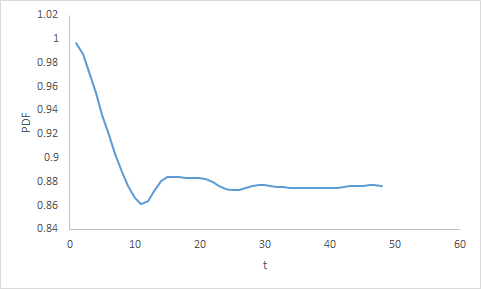
\includegraphics[width=10cm,height=5cm]{figures/PDF}
  \caption{\label{fig:PDF} Pair Distribution Function.}
\end{figure}

\section{Conclusion}
We simulated the molecular dynamics for Argon gas and calculated the temperature and energy changes using Verlet algorithm and relevant arguments and methods successfully. We learned the behavior of Argon gas through this analysis.

\appendix
\section{Characteristics of Argon}
Melting point: -189.37$^{\circ}$ C\\
Boiling point: -185.7$^{\circ}$ C\\
Latent heat of fusion (1.013 bar at melting point): 29.588 kJ/kg\\
Latent heat of vaporization (1.013 bar at boiling point): -161.14 kJ/kg\\
Critical temperature: -122.46$^{\circ}$ C\\
Triple point temperature: -189.34$^{\circ}$ C\\
Critical pressure: 48.63 bar\\
Critical density: 535.6 kgm$^{-3}$\\
Energy of first ionization: 1520 kJmol$^{-1}$\\
Energy of second ionization: 2665.8 kJmol$^{-1}$\\
Energy of third ionization: 3931 kJmol$^{-1}$\\
Density : 1.78 10$^{-3}$ gcm$^{-3}$ at 0$^{\circ}$ C\\

\end{document}
